\documentclass[a4paper,10pt]{article}
\usepackage[utf8x]{inputenc}
\usepackage[top=1.5cm, bottom=1.5cm,left=2cm,right=1.5cm]{geometry}
\usepackage{url}
\usepackage[hyperfootnotes=false]{hyperref}
\usepackage{listings}
\usepackage[nogin]{Sweave}

%opening
\title{Analysis of the \#thankcsiroforthat Twitter hashtag}
\author{Neil Saunders}
\lstset{breaklines=true}

\renewcommand*\rmdefault{phv}

\begin{document}
\Sconcordance{concordance:thankCSIROjson.tex:thankCSIROjson.Rnw:%
1 19 1 1 22 7 1 2 2 10 1 1 4 1 2 9 1 1 5 1 1 1 4 3 1 1 4 4 1 1 16 1 1 1 %
6 9 1 1 6 37 1 1 12 7 1 1 17 8 1}

\maketitle

\section{Introduction}

859 tweets with the hashtag \#thankcsiroforthat were retrieved. The text of 216 tweets was unique.

\section{Tweet frequency}
Tweets with the \#thankcsiroforthat hashtag peaked early on the first day at 161 per hour, then continued at a steady rate throughout the next day.

\begin{figure}[h]
\begin{center}
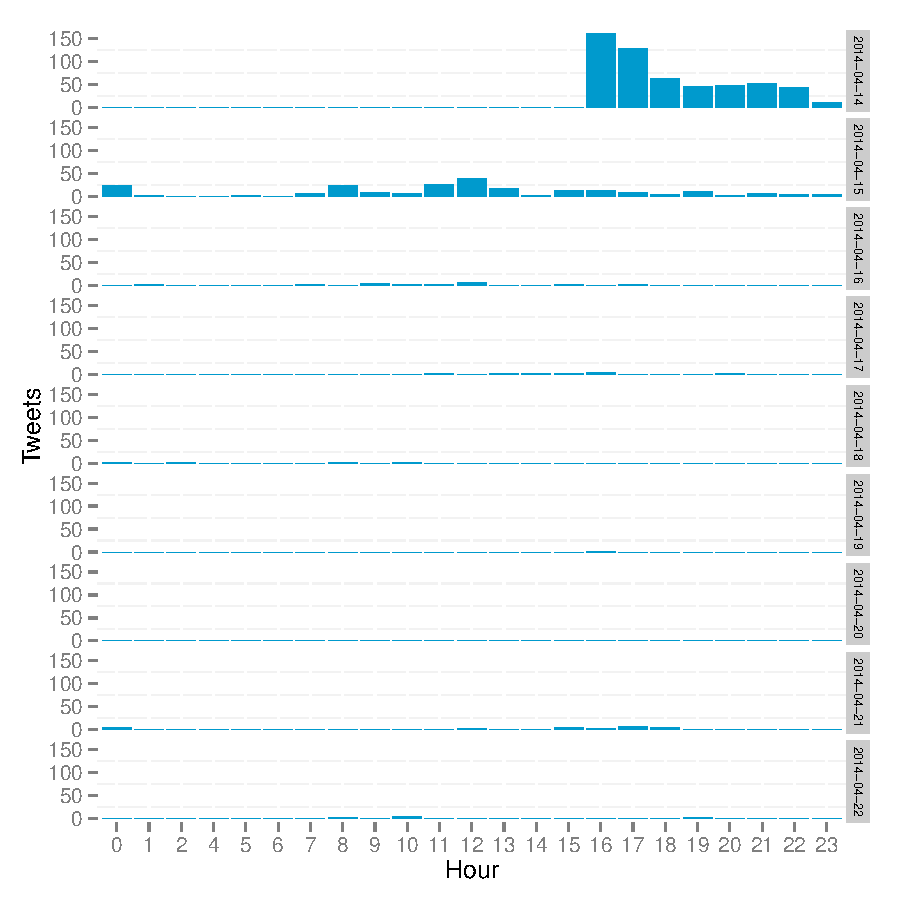
\includegraphics{thankCSIROjson-002}
\caption{\#thankcsiroforthat tweets per hour}
\end{center}
\end{figure}

\newpage

\section{Twitter users}
501 posted at least one tweet. 125 posted more than one tweet. Here are the top 20 users by tweets, with follower count.

\begin{figure}[h]
\begin{center}
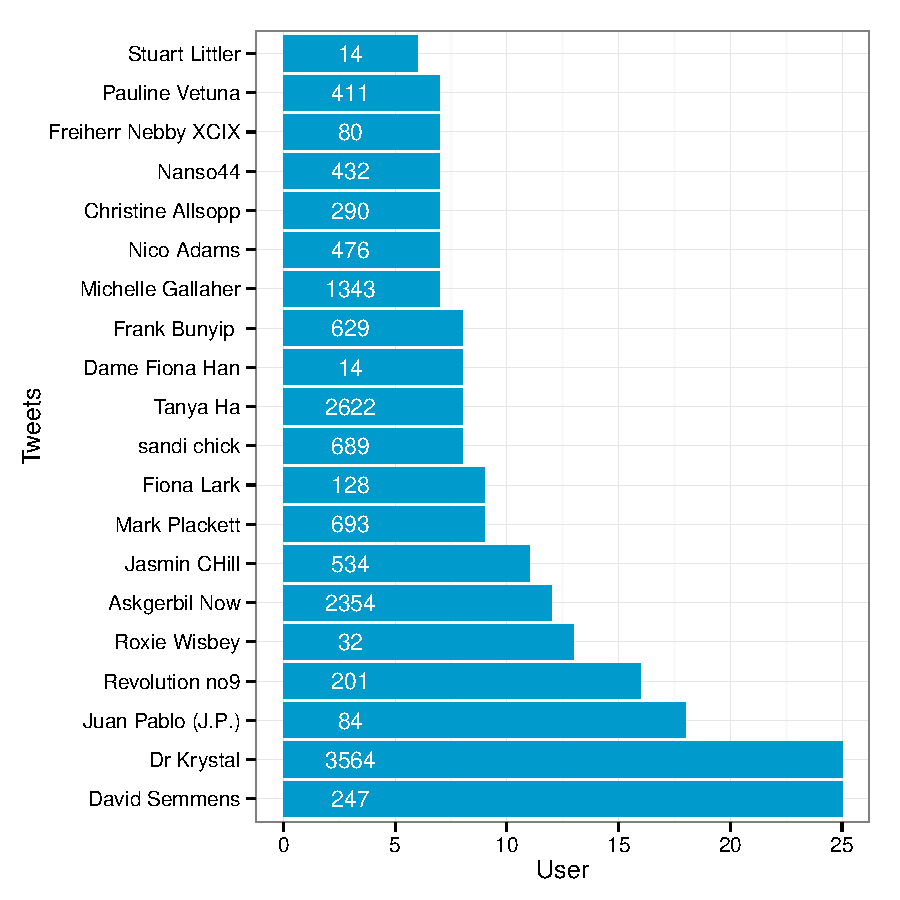
\includegraphics{thankCSIROjson-003}
\caption{Top 20 users by number of tweets; numbers (white) = followers}
\end{center}
\end{figure}

%\newpage

\section{Retweets and favourites}
Most retweets: 255.

\begin{lstlisting}
[1] "RT @tanya_plibersek: Tweeting using wifi? You should #thankcsiroforthat #auspol"\end{lstlisting}


\noindent Most favourites: 21 (Kim Carr).

\begin{lstlisting}
[1] "88 years of outstanding science, research and groundbreaking discoveries http://t.co/jCQvci6Gwp #thankcsiroforthat #auspol"\end{lstlisting}

\newpage

\section{Word frequency}

%\subsection{Using unique tweet text}

For those who like word clouds.

\begin{figure}[h]
\begin{center}

\includegraphics[scale=0.55]{thankCSIROjson-cloud.pdf}
\caption{Top 150 words appearing 3 or more times in 216 unique tweets with hashtag \#thankcsiroforthat}
\end{center}
\end{figure}


\noindent For those who like bar graphs.

\begin{figure}[h]
\begin{center}
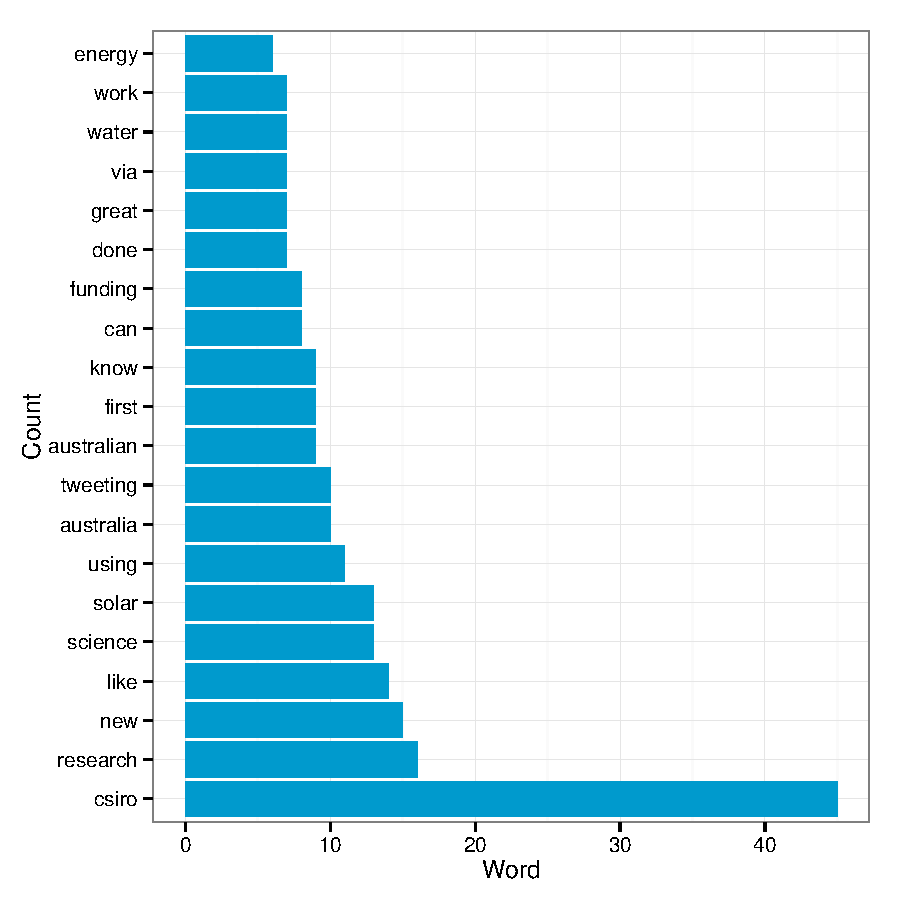
\includegraphics[scale=0.55]{thankCSIROjson-bar.pdf}
\caption{Top 20 words appearing 2 or more times in 216 unique tweets with hashtag \#thankcsiroforthat}
\end{center}
\end{figure}

\newpage

%\subsection{Using all tweet text}
%\begin{figure}[h]
%\begin{center}
%<<fig=TRUE, echo=FALSE>>=
%wordcount <- countWords(strsplit(as.character(thankcsiro$text), " "))
%wordcloud(wordcount$words, wordcount$Freq, scale = c(8, .2), min.freq = 3,
%          max.words = 150, random.order = FALSE, rot.per = .15, colors = pal2)
%@
%\end{center}
%\end{figure}
%
%\begin{figure}[h]
%\begin{center}
%<<fig=TRUE, echo=FALSE>>=
%words.20 <- head(wordcount, 20)
%words.20$words <- factor(words.20$words, levels = as.character(words.20$words))
%print(ggplot(words.20) + geom_bar(aes(words, Freq), stat = "identity", fill = "deepskyblue3") + theme_bw() + coord_flip())
%@
%\end{center}
%\end{figure}
%
%\newpage

\section{Sentiment analysis}
Disclaimer: sentiment analysis is (mostly, probably) rubbish. The methods used here are from Godbole \textit{et al.}\footnote{Godbole, N., Srinivasaiah, M. and Skiena, S. Large-Scale Sentiment Analysis for News and Blogs. Int. Conf. on Weblogs and Social Media (ICWSM 2007), Denver CO, March 26-28, 2007. \href{http://icwsm.org/papers/3--Godbole-Srinivasaiah-Skiena.pdf}{PDF}} Most tweets were classified as neutral or positive.


\begin{figure}[h]
\begin{center}
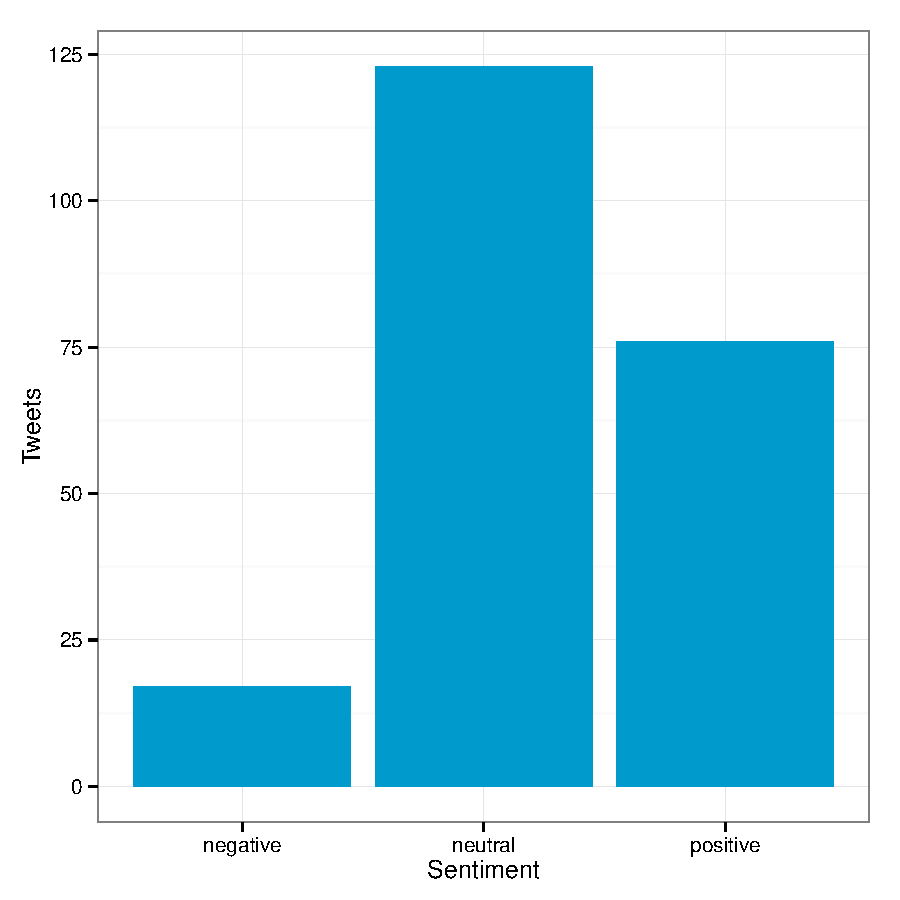
\includegraphics[scale=0.55]{thankCSIROjson-senticount.pdf}
\caption{Number of tweets classed as negative, neutral or positive sentiment in 216 unique tweets with hashtag \#thankcsiroforthat}
\end{center}
\end{figure}


\begin{figure}[h]
\begin{center}
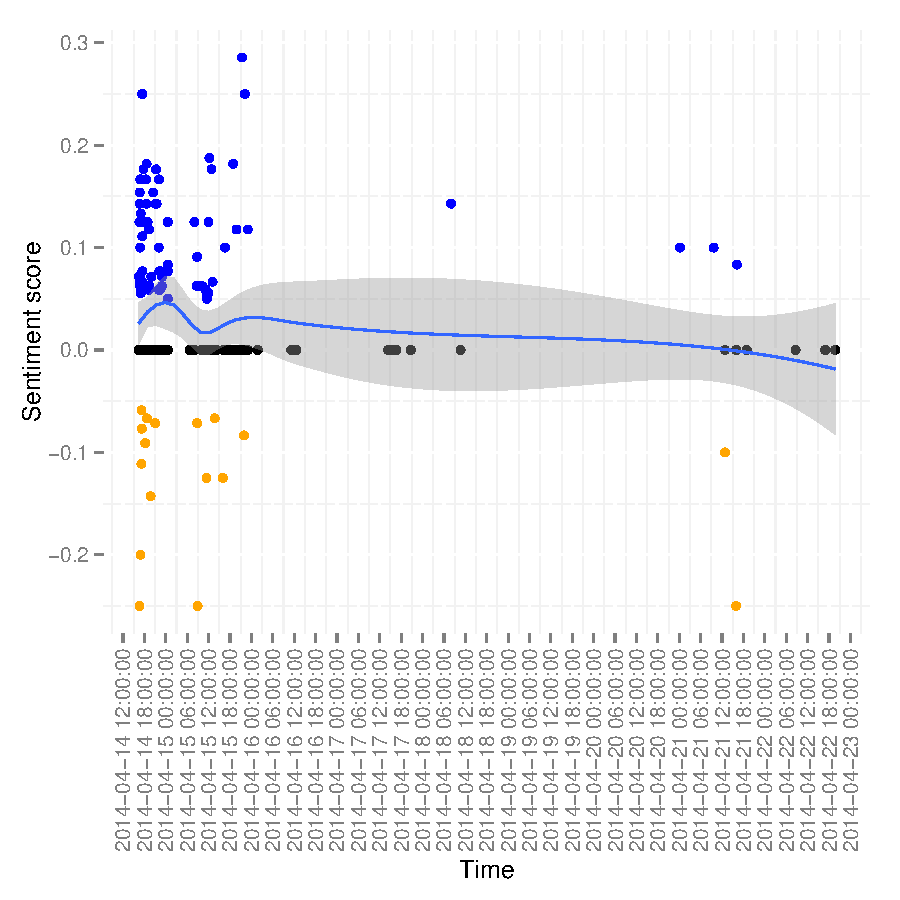
\includegraphics[scale=0.55]{thankCSIROjson-sentitime.pdf}
\caption{Tweet sentiment over time for tweets with hashtag \#thankcsiroforthat. Blue = positive, orange = negative, black = neutral.}
\end{center}
\end{figure}

\end{document}
